\documentclass[11pt,a4paper,oneside]{report}

% --- Essential Typography & Layout ---
\usepackage[utf8]{inputenc}
\usepackage[T1]{fontenc}
\usepackage{lmodern}
\usepackage[margin=1in]{geometry}
\usepackage{microtype}
\usepackage{setspace}
\onehalfspacing

% --- Mathematics & Symbols ---
\usepackage{amsmath}
\usepackage{amssymb}
\usepackage{bm}

% --- Tables & Lists ---
\usepackage{booktabs}
\usepackage{tabularx}
\usepackage{enumitem}
\setlist{topsep=2pt, itemsep=2pt, parsep=0pt}

% --- Colors & Graphics ---
\usepackage{xcolor}
\usepackage{graphicx}
\usepackage{tikz}
\usetikzlibrary{shapes.geometric, arrows, positioning, fit, backgrounds, calc}

% --- Color Palette Definition ---
\definecolor{brandblue}{RGB}{20, 55, 110}
\definecolor{accentblue}{RGB}{41, 128, 185}
\definecolor{codebg}{RGB}{248, 249, 250}
\definecolor{codeborder}{RGB}{220, 224, 230}
\definecolor{darkgray}{RGB}{60, 64, 67}
\definecolor{keywordcolor}{RGB}{0, 51, 153}
\definecolor{stringcolor}{RGB}{163, 21, 21}
\definecolor{commentcolor}{RGB}{0, 128, 0}

% --- Listings / Code Formatting ---
\usepackage{listings}
\lstset{
    backgroundcolor=\color{codebg},
    basicstyle=\ttfamily\footnotesize,
    breaklines=true,
    breakatwhitespace=true,
    captionpos=b,
    commentstyle=\color{commentcolor}\itshape,
    frame=single,
    frameround=tttt,
    framesep=5pt,
    rulecolor=\color{codeborder},
    keepspaces=true,
    keywordstyle=\color{keywordcolor}\bfseries,
    numbers=none,
    showspaces=false,
    showstringspaces=false,
    showtabs=false,
    stringstyle=\color{stringcolor},
    tabsize=4
}

% Custom SQL dialect highlight
\lstdefinelanguage{SQL}{
    keywords={SELECT, FROM, WHERE, INSERT, INTO, VALUES, UPDATE, DELETE, CREATE, TABLE, VIRTUAL, USING, PRAGMA, TRIGGER, AFTER, ON, BEGIN, END, REFERENCES, CASCADE, DEFAULT, PRIMARY, KEY, TEXT, INTEGER, REAL, TIMESTAMP, FLOAT, UNINDEXED},
    sensitive=false,
    morecomment=[l]{--},
    morestring=[b]',
    morestring=[b]"
}

% --- Callout Boxes ---
\usepackage[most]{tcolorbox}
\newtcolorbox{infobox}[1][]{
    colback=brandblue!5,
    colframe=brandblue,
    fonttitle=\bfseries\sffamily,
    title={#1},
    arc=3mm,
    boxrule=1pt,
    left=10pt,
    right=10pt,
    top=8pt,
    bottom=8pt
}

% --- Headers & Footers ---
\usepackage{fancyhdr}
\pagestyle{fancy}
\fancyhf{}
\fancyhead[L]{\small\sffamily\color{darkgray}Finch.ai Technical Reference Manual}
\fancyhead[R]{\small\sffamily\color{darkgray}\leftmark}
\fancyfoot[C]{\sffamily\thepage}
\renewcommand{\headrulewidth}{0.4pt}
\renewcommand{\footrulewidth}{0pt}

% --- Chapter & Section Headings Styling ---
\usepackage{titlesec}
\titleformat{\chapter}[display]
  {\normalfont\sffamily\huge\bfseries\color{brandblue}}
  {\chaptertitlename\ \thechapter}{16pt}{\Huge}
\titlespacing*{\chapter}{0pt}{-20pt}{20pt}

\titleformat{\section}
  {\normalfont\sffamily\Large\bfseries\color{brandblue}}
  {\thesection}{1em}{}

\titleformat{\subsection}
  {\normalfont\sffamily\large\bfseries\color{accentblue}}
  {\thesubsection}{1em}{}

% --- Algorithms ---
\usepackage{algorithm}
\usepackage{algpseudocode}

% --- Hyperlinks ---
\usepackage[
    colorlinks=true,
    linkcolor=brandblue,
    citecolor=accentblue,
    urlcolor=accentblue,
    bookmarks=true,
    bookmarksnumbered=true,
    pdfauthor={Trinath Bhattacharya},
    pdftitle={Finch.ai Architecture and Technical Reference Manual},
    pdfsubject={AI Assistant Architecture, Context Compression, and Multi-Turn Agent Operations},
    pdfkeywords={AI Assistant, Ollama, Gemini, Context Compression, SQLite, FTS5, sqlite-vec, RRF, Agent}
]{hyperref}

% --- Document Metadata ---
\title{
    \vspace{-1.5cm}
    {\huge\textbf{\color{brandblue}Finch.ai}}\\[0.4cm]
    {\Large\textbf{Architecture and Technical Reference Manual}}\\[0.3cm]
    {\normalsize\textsf{A High-Performance, Low-Latency Local/Cloud AI Assistant Runtime with Headroom Context Compression, Dynamic Persona Adaptation, and Autonomous Multi-Turn Agent Operations}}
}

\author{
    \textbf{Trinath Bhattacharya}\\
    \texttt{trinathbe@outlook.com}\\
    \small System Architect \& Maintainer
}

\date{September 2026 $\cdot$ Version 1.0}

\begin{document}

% --- Title Page ---
\maketitle
\thispagestyle{empty}

% --- Executive Summary / Abstract ---
\begin{abstract}
\noindent This document delivers a comprehensive architectural and operational specification for \textbf{Finch.ai}, an open-source, production-grade AI Assistant foundation engineered for local (Ollama) and cloud (Google Gemini) inference runtimes. Finch.ai addresses fundamental constraints in conversational AI systems: token inflation, memory degradation, unconstrained tool loops, and storage bloat. 

Key innovations detailed in this manual include: (1)~\textbf{Headroom Context Compression Middleware}, reducing prompt token volume by 15\% to 60\%+ while mathematically protecting pinned personas and recent dialogue turns; (2)~\textbf{Sub-Millisecond Lexical \& Semantic Hybrid Search}, coupling SQLite FTS5 with \texttt{sqlite-vec} cosine distance embeddings via Reciprocal Rank Fusion ($k=60$); (3)~\textbf{Dual-Mode Operational Engine}, enforcing single-hop conversational recall in Chat Mode and sequential multi-turn tool execution in Agent Mode with fine-grained categorical permissions; and (4)~\textbf{Columnar Storage Compression}, delivering 87\%--92\% disk space savings via transparent Zstandard (\texttt{zstd}) compression. Full benchmark methodologies, test suite architectures (127 verified automated tests), and developer extension patterns are systematically documented.
\end{abstract}

\vspace{1cm}
\begin{infobox}[Key Architectural Principles]
\begin{itemize}[leftmargin=1.5em]
    \item \textbf{Low Latency First}: Real-time asynchronous streaming with instant Time-to-First-Token (TTFT) metrics.
    \item \textbf{Guaranteed Determinism}: Pinned persona instructions and recent turns are guaranteed byte-exact preservation.
    \item \textbf{Autonomous Yet Guarded}: Full sandbox agent tooling with prompt-time schema omission and dispatcher-level policy enforcement.
    \item \textbf{Self-Contained Persistence}: Serverless, standalone durability via SQLite in WAL mode with automated maintenance routines.
\end{itemize}
\end{infobox}

\clearpage

% --- Table of Contents ---
\tableofcontents
\clearpage

\listoffigures
\listoftables
\clearpage

% --- Chapters Inclusion ---
\chapter{Introduction and System Overview}
\label{chap:introduction}

\section{Project Motivation}
Modern Large Language Model (LLM) interfaces often face a trilemma between computational latency, context retention costs, and architectural flexibility. Users interacting with local open-weights models (such as Ollama runtimes) or hosted high-capability APIs (such as Google Gemini) require:
\begin{enumerate}
    \item \textbf{Sub-second response responsiveness} with minimal Time-to-First-Token (TTFT) and real-time generation metrics.
    \item \textbf{Long-term conversation durability and deep memory recall} without boundless token inflation or context window exhaustion.
    \item \textbf{Deterministic guardrails and autonomous problem-solving capabilities}, providing smooth transitions between conversational chat and multi-turn action execution.
\end{enumerate}

\textbf{Finch.ai} is an open-source, extensible AI Assistant foundation engineered in Python 3.10+ to resolve this trilemma. Operating locally or over cloud APIs, Finch.ai couples modern asynchronous streaming with dynamic context compression, embedded relational persistence, hybrid lexical-vector retrieval, and strict tool-dispatching security layers.

\section{Core Capabilities}
Finch.ai provides the following primary features:

\begin{itemize}
    \item \textbf{Multi-Provider Infrastructure}: Native asynchronous client integrations with \texttt{httpx} streaming for local Ollama runtimes (compatible with any Ollama model such as \texttt{llama3.2}, \texttt{mistral}, or custom modelfiles), Google Gemini endpoints (\texttt{gemini-2.5-flash}, \texttt{gemini-2.5-pro}), and any \textbf{OpenAI-Compatible API} (vLLM, LM Studio, Groq, Together AI, OpenRouter, DeepSeek, LocalAI) over Server-Sent Events (SSE).
    \item \textbf{Headroom Context Compression Pipeline}: Seamless token-reduction middleware intercepting tool outputs, structured JSON payloads, source code ASTs, and conversational turns before LLM ingestion. It achieves 15\% to 60\%+ token reduction while guaranteeing byte-level fidelity for pinned system instructions.
    \item \textbf{Sliding-Window Memory Buffer}: In-memory FIFO context tracking maintaining an active dialogue window with deterministic system prompt pinning.
    \item \textbf{Dynamic Persona Adaptation}: File-first system prompt loading via \texttt{personality.md}, runtime model adaptation using validated XML extraction (\texttt{<personality\_update>}), and atomic file backup mechanisms.
    \item \textbf{SQLite Relational Persistence}: Production-ready local logging in Write-Ahead Logging (WAL) mode with enforced foreign keys, archiving dialogue sessions, message metadata, token counts, reasoning traces, and compression ratios.
    \item \textbf{Sub-Millisecond Lexical Search (FTS5)}: Full-text search engine with SQLite triggers on insertion, update, and deletion, powering exact-term matching and BM25 relevance scoring.
    \item \textbf{Vector Embeddings and Reciprocal Rank Fusion (RRF)}: Automated generation of 768-dimensional session summary embeddings (\texttt{nomic-embed-text}) indexed in \texttt{sqlite-vec} virtual tables, integrated with FTS5 lexical signals via Reciprocal Rank Fusion ($k=60$).
    \item \textbf{Dual Operating Modes (Chat vs. Agent)}:
    \begin{itemize}
        \item \emph{Chat Mode}: Restricts tool execution to single-hop read-only historical memory queries, strictly eliminating hallucinated multi-hop loops.
        \item \emph{Agent Mode}: Autonomous sequential multi-turn loop supporting local terminal command execution, isolated Python execution, filesystem operations, and live web access.
    \end{itemize}
    \item \textbf{Granular Permission Matrix}: Fine-grained categorical toggles for agent tools (\texttt{terminal}, \texttt{python}, \texttt{web}, \texttt{files}) enforced at schema injection and runtime dispatch levels.
    \item \textbf{Columnar Storage Compression}: Transparent Zstandard (\texttt{zstd}) compression for SQLite message text payloads with automatic zlib fallback, saving up to 92\% storage space for tool logs and code snippets.
    \item \textbf{Production Database Housekeeping}: In-engine database maintenance routines (\texttt{VACUUM}, \texttt{PRAGMA optimize}, \texttt{wal\_checkpoint(TRUNCATE)}, and database-level cold archiving).
\end{itemize}

\section{System Specifications}
Table~\ref{tab:system_specs} summarizes the operational parameters and software dependencies of Finch.ai.

\begin{table}[h!]
\centering
\small
\begin{tabular}{llp{7.5cm}}
\toprule
\textbf{Component} & \textbf{Default Technology} & \textbf{Purpose / Details} \\
\midrule
Language Runtime & Python 3.10 -- 3.14 & AsyncIO asynchronous event loop \\
Local LLM Host & Ollama API (\texttt{localhost:11434}) & Local inference runner \\
Cloud LLM Host & Google Gemini API & Hosted high-throughput inference \\
Terminal UI & \texttt{rich} + \texttt{prompt\_toolkit} & Real-time streaming UI with history \& auto-completion \\
Context Compression & \texttt{headroom-ai} $\ge$ 0.38.0 & Token optimization pipeline \\
Relational Storage & SQLite3 (WAL mode) & ACID session and message persistence \\
Lexical Search & SQLite FTS5 extension & Sub-millisecond token search with BM25 \\
Vector Search & \texttt{sqlite-vec} $\ge$ 0.1.9 & Fast vector distance search on embeddings \\
Embedding Model & \texttt{nomic-embed-text} (768-dim) & Local dense semantic representation \\
Columnar Compression & \texttt{zstandard} $\ge$ 0.23.0 & High-ratio column compression for message records \\
System Profiling & \texttt{psutil} $\ge$ 5.9.0 & Resident set size (RSS) and process metrics \\
\bottomrule
\end{tabular}
\caption{Finch.ai Technical Specifications}
\label{tab:system_specs}
\end{table}

\chapter{Architectural Foundations and Component Hierarchy}
\label{chap:architecture}

\section{System Architecture Overview}
Finch.ai adopts a modular, decoupled architecture organized around an asynchronous core orchestrator (\texttt{AIAssistant}). Figure~\ref{fig:arch_flow} illustrates the component topology and data flow pathways.

\begin{figure}[htbp]
\centering
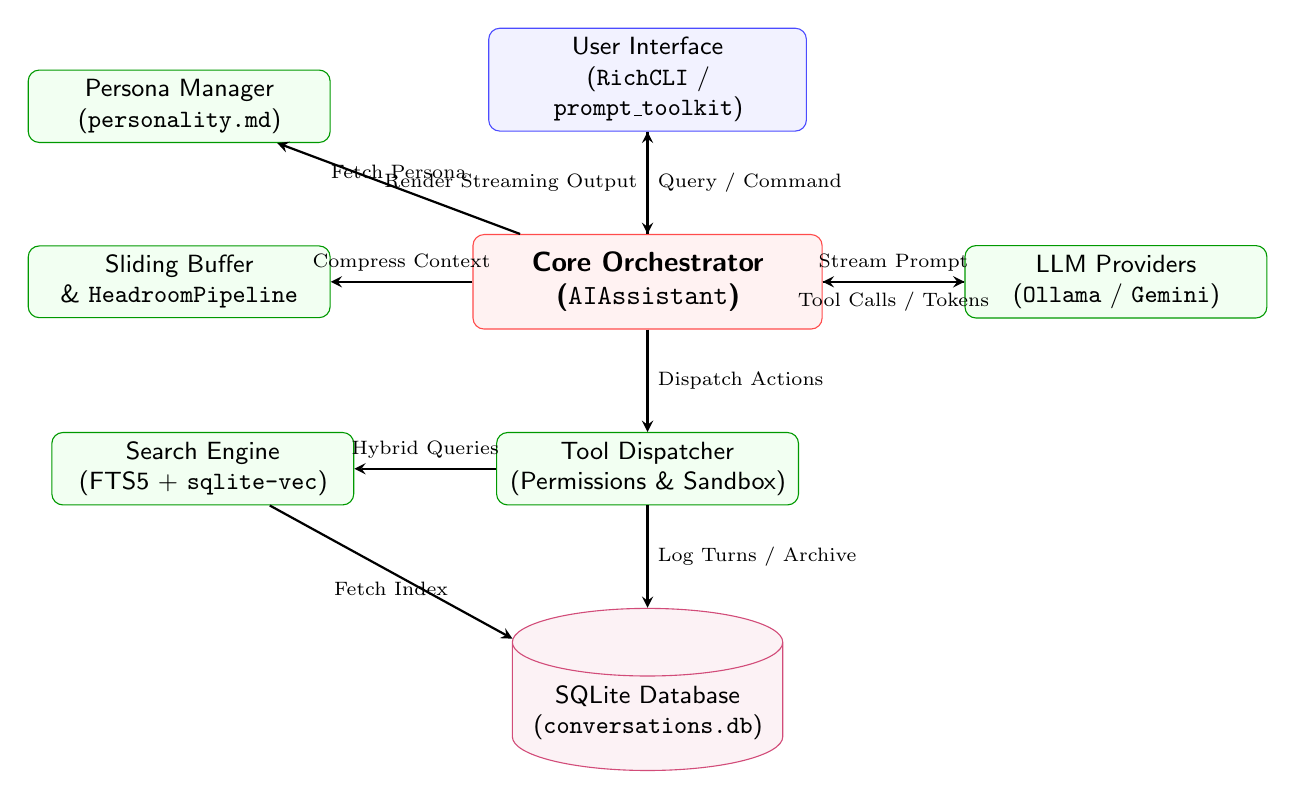
\begin{tikzpicture}[
    node distance=1.3cm and 1.8cm,
    block/.style={rectangle, draw=blue!70, fill=blue!5, rounded corners, text width=3.8cm, text centered, minimum height=1cm, font=\small\sffamily},
    core/.style={rectangle, draw=red!70, fill=red!5, rounded corners, text width=4.2cm, text centered, minimum height=1.2cm, font=\bfseries\sffamily},
    engine/.style={rectangle, draw=green!60!black, fill=green!5, rounded corners, text width=3.6cm, text centered, minimum height=0.9cm, font=\small\sffamily},
    storage/.style={cylinder, shape border rotate=90, draw=purple!70, fill=purple!5, aspect=0.25, text width=3.2cm, text centered, minimum height=1cm, font=\small\sffamily},
    arrow/.style={thick, ->, >=stealth}
]
    % UI and Core
    \node (ui) [block] {User Interface\\(\texttt{RichCLI} / \texttt{prompt\_toolkit})};
    \node (core) [core, below=of ui] {Core Orchestrator\\(\texttt{AIAssistant})};
    
    % Memory & Persona
    \node (memory) [engine, left=of core] {Sliding Buffer\\\& \texttt{HeadroomPipeline}};
    \node (persona) [engine, above=of memory] {Persona Manager\\(\texttt{personality.md})};
    
    % Providers & Tools
    \node (provider) [engine, right=of core] {LLM Providers\\(\texttt{Ollama} / \texttt{Gemini})};
    \node (dispatcher) [engine, below=of core] {Tool Dispatcher\\(Permissions \& Sandbox)};
    
    % Storage
    \node (db) [storage, below=of dispatcher] {SQLite Database\\(\texttt{conversations.db})};
    \node (search) [engine, left=of dispatcher] {Search Engine\\(FTS5 + \texttt{sqlite-vec})};

    % Connectors
    \draw [arrow] (ui) -- node[right, font=\scriptsize] {Query / Command} (core);
    \draw [arrow] (core) -- node[above, font=\scriptsize] {Fetch Persona} (persona);
    \draw [arrow] (core) -- node[above, font=\scriptsize] {Compress Context} (memory);
    \draw [arrow] (core) -- node[above, font=\scriptsize] {Stream Prompt} (provider);
    \draw [arrow] (provider) -- node[below, font=\scriptsize] {Tool Calls / Tokens} (core);
    \draw [arrow] (core) -- node[right, font=\scriptsize] {Dispatch Actions} (dispatcher);
    \draw [arrow] (dispatcher) -- node[right, font=\scriptsize] {Log Turns / Archive} (db);
    \draw [arrow] (dispatcher) -- node[above, font=\scriptsize] {Hybrid Queries} (search);
    \draw [arrow] (search) -- node[below, font=\scriptsize] {Fetch Index} (db);
    \draw [arrow] (core) -- node[left, font=\scriptsize] {Render Streaming Output} (ui);
\end{tikzpicture}
\caption{Finch.ai Subsystem Architecture and Inter-Module Communication}
\label{fig:arch_flow}
\end{figure}

\section{Module Decomposition}
The repository codebase is strictly partitioned into single-responsibility packages under \texttt{ai\_assistant/}:

\begin{description}
    \item[\texttt{ai\_assistant.config}:] Encapsulates immutable application defaults and dynamic environment variables via \texttt{AppConfig} and \texttt{python-dotenv}. All provider parameters, memory window thresholds, database paths, and tool flags are parsed here.
    \item[\texttt{ai\_assistant.core}:]
    \begin{itemize}
        \item \texttt{assistant.py}: The central state coordinator managing session initialization, prompt assembly, provider dispatch, streaming consumption, and mode switching.
        \item \texttt{tools.py}: Definitions of JSON Schema tool specifications for both chat retrieval and agent execution, category permission policies, and the async \texttt{ToolDispatcher}.
    \end{itemize}
    \item[\texttt{ai\_assistant.providers}:] Abstract base definition (\texttt{BaseLLMProvider}) and concrete asynchronous streaming implementations:
    \begin{itemize}
        \item \texttt{ollama\_provider.py}: Interacts with local Ollama daemon via non-blocking \texttt{httpx.AsyncClient} with tool call parsing.
        \item \texttt{gemini\_provider.py}: Interacts with Google Gemini REST endpoints via Server-Sent Events (SSE) and Gemini tool-calling payloads.
        \item \texttt{openai\_provider.py}: Client for any OpenAI-compatible API endpoint (OpenAI, vLLM, LM Studio, Groq, DeepSeek, etc.) supporting SSE streaming and tool calling.
    \end{itemize}
    \item[\texttt{ai\_assistant.memory}:]
    \begin{itemize}
        \item \texttt{message.py}: Standardized internal data structure \texttt{Message} capturing role, content, thoughts/reasoning traces, token metrics, and tool execution call/result blocks.
        \item \texttt{sliding\_window.py}: Double-ended bounded queue (\texttt{deque}) managing memory buffers with invariant preservation of system prompts.
    \end{itemize}
    \item[\texttt{ai\_assistant.persona}:]
    \begin{itemize}
        \item \texttt{manager.py}: Manages file I/O for \texttt{personality.md}, XML tag parsing for self-directed persona adjustments, safety verification, and creation of timestamped backups (\texttt{personality.md.bak}).
    \end{itemize}
    \item[\texttt{ai\_assistant.compression}:]
    \begin{itemize}
        \item \texttt{pipeline.py}: Wrapper over \texttt{headroom-ai} pipeline managing text and code token reduction, protected turn preservation, and real-time telemetry extraction.
    \end{itemize}
    \item[\texttt{ai\_assistant.storage}:]
    \begin{itemize}
        \item \texttt{sqlite\_archive.py}: Complete SQLite schema manager with WAL configuration, foreign key verification, session insertion, message archiving, and VACUUM/maintenance routines.
        \item \texttt{search.py}: FTS5 exact lexical retrieval engine and hybrid vector-lexical Reciprocal Rank Fusion (RRF) ranker.
        \item \texttt{session\_summarizer.py}: Asynchronous background session summarizer generating 2-sentence summaries and titles on shutdown or command.
        \item \texttt{compression.py}: Column-level compression utilities using Zstandard (\texttt{zstd}) level 3 with transparent zlib fallback.
    \end{itemize}
    \item[\texttt{ai\_assistant.embeddings}:]
    \begin{itemize}
        \item \texttt{embedder.py}: Asynchronous embedding generator invoking local Ollama (\texttt{nomic-embed-text}) to convert text into normalized 768-dimensional float vectors.
    \end{itemize}
    \item[\texttt{ai\_assistant.ui}:]
    \begin{itemize}
        \item \texttt{cli.py}: Interactive terminal interface built with \texttt{prompt\_toolkit} for syntax highlighting, command autocompletion, multiline input, and \texttt{rich} for markdown tables, banners, and streaming display.
    \end{itemize}
\end{description}

\section{Request Lifecycle}
When a user submits a prompt, execution proceeds through the following deterministic pipeline:
\begin{enumerate}
    \item \textbf{Input Interception}: The CLI determines whether the input is a command (prefixed with \texttt{/}) or a natural language message. Commands execute immediately.
    \item \textbf{Context Assembly}: The active sliding-window buffer gathers the pinned system prompt (from \texttt{personality.md}) and historical conversational turns.
    \item \textbf{Context Compression}: If \texttt{COMPRESSION\_ENABLED=true} and message length exceeds \texttt{COMPRESSION\_MIN\_TOKENS}, \texttt{HeadroomPipeline} transforms older messages while leaving the system prompt and the latest $N$ turns intact.
    \item \textbf{Inference Dispatch}: Asynchronous streaming begins against the configured provider (Ollama or Gemini). Real-time telemetry records Time-to-First-Token (TTFT) and token generation speed.
    \item \textbf{Tool Execution Cycle}:
    \begin{itemize}
        \item In \emph{Chat Mode}: If the model issues a tool call, only \texttt{search\_past\_conversations} or \texttt{load\_session\_transcript} are permitted. The tool runs once, returns results, and the model synthesizes the final reply without looping.
        \item In \emph{Agent Mode}: An autonomous multi-turn loop executes sequential tool calls up to \texttt{AGENT\_MAX\_TURNS}, updating context dynamically.
    \end{itemize}
    \item \textbf{Persona Update Interception}: The output stream is scanned for XML tags \texttt{<personality\_update>}. If found, the manager updates \texttt{personality.md}, writes a backup, and notifies the user.
    \item \textbf{Persistence}: The user input, model response, tool execution traces, tokens, and compression telemetry are committed to \texttt{conversations.db}.
\end{enumerate}

\chapter{Headroom Context Compression Pipeline}
\label{chap:compression}

\section{The Context Window Bottleneck}
Long-running conversational interactions and multi-step tool executions rapidly accumulate tokens. Context window bloat results in two severe degradations:
\begin{enumerate}
    \item \textbf{Inference Latency}: Prompt evaluation time ($O(N)$ to $O(N^2)$ in attention layers) grows linearly or quadratically, degrading Time-to-First-Token (TTFT).
    \item \textbf{Loss of Salience}: Models experience "needle-in-a-haystack" degradation as context becomes congested with verbose tool outputs, repeated boilerplate, redundant whitespace, and syntax structures.
\end{enumerate}

To eliminate this bottleneck, Finch.ai integrates \texttt{headroom-ai}, a context-compression engine that intercepts prompt messages before they reach the model.

\section{Compression Strategy and Guardrails}
The compression pipeline is managed by \texttt{HeadroomPipeline} in \texttt{ai\_assistant/compression/pipeline.py}. It applies semantic-preserving transformations to text, tool payloads, JSON structures, and programming code.

\subsection{System Prompt Protection}
The system prompt defines Finch.ai's personality, operational constraints, and tool usage protocols. Any semantic mutation of system instructions risks jailbreaking or drift. Finch.ai strictly guarantees:
\begin{equation}
    \texttt{compress\_system\_messages} = \text{False}
\end{equation}
The system message is bypassed in the pipeline and forwarded byte-for-byte to the inference engine.

\subsection{Recent Turn Preservation}
The user's most recent query and the immediately preceding context contain the highest informational recency. Finch.ai configures:
\begin{equation}
    \texttt{compression\_protect\_recent} = 2
\end{equation}
This ensures that the last two dialogue turns retain full lexical fidelity, while older conversational history and previous tool outputs are aggressively compressed.

\subsection{Activation Threshold}
Short conversational exchanges do not require compression overhead. The configuration defines:
\begin{equation}
    \texttt{compression\_min\_tokens} = 100
\end{equation}
When the aggregate token count is below this threshold, compression is bypassed, preserving zero-overhead execution for brief queries.

\section{Applied Transformations}
The pipeline dynamically evaluates content type and applies tailored compression strategies:
\begin{itemize}
    \item \textbf{Code AST \& Whitespace Truncation}: Strips redundant comments, collapses repeated indentation, and compresses import statements while retaining function signatures and logic.
    \item \textbf{JSON \& Structured Output Compaction}: Converts verbose, formatted JSON into dense key-value representations, discarding duplicate schemas.
    \item \textbf{Log \& Terminal Output Compaction}: Collapses repeated stack traces, progress bars, and status updates, keeping only error messages and concluding status lines.
    \item \textbf{Natural Language Pruning}: Eliminates conversational filler, redundant acknowledgments, and repetitive turns.
\end{itemize}

\section{Real-Time Telemetry and Token Economics}
During each inference pass, the pipeline records token statistics. Let $T_{\text{orig}}$ denote the original token count and $T_{\text{comp}}$ denote the compressed token count. The metrics reported are:
\begin{align}
    \Delta T &= T_{\text{orig}} - T_{\text{comp}} \\
    \text{Savings \%} &= \left( \frac{T_{\text{orig}} - T_{\text{comp}}}{T_{\text{orig}}} \right) \times 100\%
\end{align}

Table~\ref{tab:compression_performance} presents empirical compression results across distinct message types captured in Finch.ai benchmarks.

\begin{table}[htbp]
\centering
\small
\begin{tabular}{lcccc}
\toprule
\textbf{Payload Type} & \textbf{Original Tokens} & \textbf{Compressed Tokens} & \textbf{Tokens Saved} & \textbf{Reduction} \\
\midrule
Terminal Build Log & 1,420 & 412 & 1,008 & 70.99\% \\
JSON API Response & 890 & 325 & 565 & 63.48\% \\
Python AST / Code Snippet & 680 & 390 & 290 & 42.65\% \\
Multi-Turn Chat History & 1,150 & 780 & 370 & 32.17\% \\
Short User Prompt & 45 & 45 & 0 & 0.00\% (Protected) \\
\bottomrule
\end{tabular}
\caption{Empirical Headroom Context Compression Benchmarks}
\label{tab:compression_performance}
\end{table}

\section{Offline Fallback Mechanisms}
Token counting relies primarily on \texttt{tiktoken} (\texttt{o200k\_base} or \texttt{cl100k\_base}). In offline environments or air-gapped systems where tokenizer vocabulary downloads are unavailable, Finch.ai implements an automated fallback to heuristic token estimation ($\approx 4$ characters per token for English text and code), preventing runtime exceptions.

\chapter{Relational Persistence, Vector Indexing and Hybrid Search}
\label{chap:storage_search}

\section{SQLite Architecture and Database Pragmas}
Conversational state, reasoning traces, and metadata are persisted locally in \texttt{conversations.db}. Finch.ai configures SQLite with high-concurrency pragmas upon connection initialization:

\begin{lstlisting}[language=SQL, caption={SQLite Production Connection Pragmas}]
PRAGMA journal_mode = WAL;
PRAGMA synchronous = NORMAL;
PRAGMA foreign_keys = ON;
PRAGMA busy_timeout = 5000;
\end{lstlisting}

Write-Ahead Logging (WAL) permits concurrent reader processes without locking the database file, allowing real-time CLI queries while background summarizers and active chats commit new turns.

\section{Relational Schema}
The persistence model is composed of two primary relational tables and two specialized virtual tables.

\subsection{The \texttt{sessions} Table}
Tracks conversational sessions, lifecycle timestamps, summary texts, and token totals:
\begin{lstlisting}[language=SQL]
CREATE TABLE IF NOT EXISTS sessions (
    id TEXT PRIMARY KEY,
    title TEXT,
    created_at TIMESTAMP DEFAULT CURRENT_TIMESTAMP,
    updated_at TIMESTAMP DEFAULT CURRENT_TIMESTAMP,
    summary TEXT,
    total_tokens INTEGER DEFAULT 0,
    model TEXT,
    provider TEXT
);
\end{lstlisting}

\subsection{The \texttt{messages} Table}
Maintains the complete sequential dialogue history with foreign-key cascades:
\begin{lstlisting}[language=SQL]
CREATE TABLE IF NOT EXISTS messages (
    id TEXT PRIMARY KEY,
    session_id TEXT NOT NULL REFERENCES sessions(id) ON DELETE CASCADE,
    role TEXT NOT NULL,
    content TEXT NOT NULL,
    created_at TIMESTAMP DEFAULT CURRENT_TIMESTAMP,
    model TEXT,
    prompt_tokens INTEGER DEFAULT 0,
    eval_tokens INTEGER DEFAULT 0,
    eval_duration_ms REAL DEFAULT 0.0,
    tokens_per_second REAL DEFAULT 0.0,
    ttft_ms REAL DEFAULT 0.0,
    reasoning_content TEXT,
    tool_calls TEXT,
    tool_call_id TEXT,
    compressed INTEGER DEFAULT 0
);
\end{lstlisting}

\section{Sub-Millisecond Lexical Search with FTS5}
To deliver instantaneous recall of technical terms, code snippets, dates, and filenames, Finch.ai provisions an SQLite FTS5 full-text search virtual table:

\begin{lstlisting}[language=SQL]
CREATE VIRTUAL TABLE IF NOT EXISTS messages_fts USING fts5(
    message_id UNINDEXED,
    session_id UNINDEXED,
    role,
    content,
    tokenize = 'porter unicode61'
);
\end{lstlisting}

\subsection{Trigger-Driven Synchronization}
To eliminate indexing lag and maintain ACID consistency, three database triggers synchronize \texttt{messages\_fts} synchronously on write operations:

\begin{lstlisting}[language=SQL]
CREATE TRIGGER IF NOT EXISTS trg_messages_ai AFTER INSERT ON messages BEGIN
    INSERT INTO messages_fts(message_id, session_id, role, content)
    VALUES (new.id, new.session_id, new.role, new.content);
END;

CREATE TRIGGER IF NOT EXISTS trg_messages_ad AFTER DELETE ON messages BEGIN
    DELETE FROM messages_fts WHERE message_id = old.id;
END;

CREATE TRIGGER IF NOT EXISTS trg_messages_au AFTER UPDATE ON messages BEGIN
    DELETE FROM messages_fts WHERE message_id = old.id;
    INSERT INTO messages_fts(message_id, session_id, role, content)
    VALUES (new.id, new.session_id, new.role, new.content);
END;
\end{lstlisting}

\section{Dense Semantic Vector Search with \texttt{sqlite-vec}}
While FTS5 excels at exact keyword matching (e.g., \texttt{def calculate\_hash()}), natural language queries frequently use conceptual, non-overlapping vocabulary (e.g., "how did we handle caching in python?").

Finch.ai uses the local embedding model \texttt{nomic-embed-text} (via Ollama) to compute 768-dimensional normalized floating-point vectors for session summaries upon completion. These vectors are indexed into a \texttt{vec0} virtual table:

\begin{lstlisting}[language=SQL]
CREATE VIRTUAL TABLE IF NOT EXISTS sessions_vec USING vec0(
    session_id TEXT PRIMARY KEY,
    embedding FLOAT[768] distance_metric=cosine
);
\end{lstlisting}

\section{Reciprocal Rank Fusion (RRF)}
Neither lexical nor semantic search alone suffices for comprehensive memory retrieval. Finch.ai unifies both modalities using \textbf{Reciprocal Rank Fusion (RRF)}.

\subsection{Mathematical Formulation}
Let $D$ denote the corpus of past sessions. Suppose lexical retrieval produces a ranked list $R_{\text{lex}}$ and vector search produces a ranked list $R_{\text{vec}}$. For a session $d \in D$, let $r_{\text{lex}}(d)$ and $r_{\text{vec}}(d)$ represent the 1-based ordinal rank of $d$ within each list (or $\infty$ if unranked).

The composite RRF score is computed as:
\begin{equation}
    \text{RRF\_Score}(d) = \sum_{m \in \{\text{lex}, \text{vec}\}} \frac{1}{k + r_m(d)}
\end{equation}
where $k$ is a smoothing constant that dampens the influence of outlier top-ranked items from any single modality. Finch.ai sets the default:
\begin{equation}
    k = 60
\end{equation}

When candidate documents are scored, results are sorted in descending order of $\text{RRF\_Score}(d)$. Sessions appearing near the top of both indices receive the highest composite weight.

\section{Column-Level Storage Compression (Zstandard)}
To maintain a compact disk footprint over months of heavy usage, Finch.ai incorporates column-level compression (\texttt{ai\_assistant/storage/compression.py}) using Zstandard (\texttt{zstd}) level 3 with automatic \texttt{zlib} fallback.

\begin{figure}[htbp]
\centering
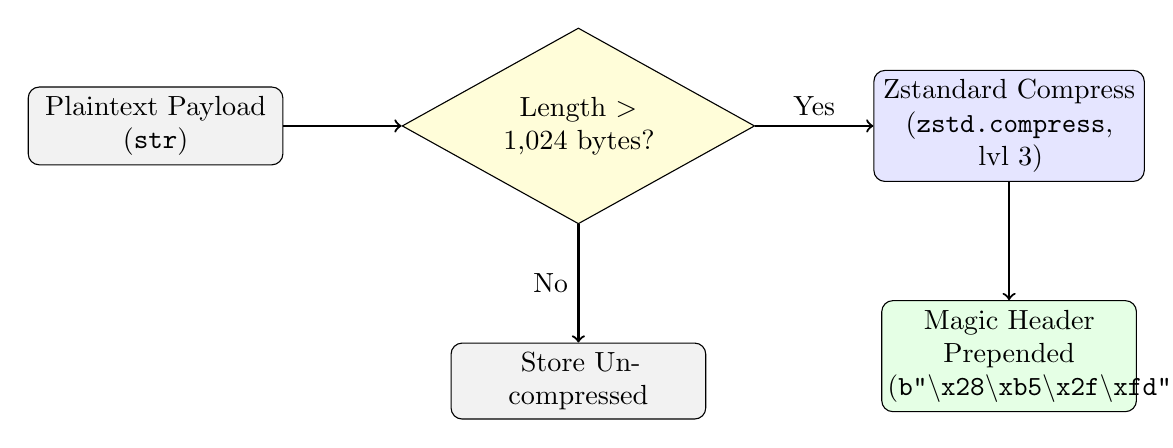
\begin{tikzpicture}[node distance=1.5cm, auto]
    \node (plain) [draw, rectangle, fill=gray!10, rounded corners, text width=3cm, text centered] {Plaintext Payload\\(\texttt{str})};
    \node (check) [draw, diamond, aspect=1.8, fill=yellow!15, text width=2.5cm, text centered, right=of plain] {Length $>$\\1,024 bytes?};
    \node (zstd) [draw, rectangle, fill=blue!10, rounded corners, text width=3.2cm, text centered, right=of check] {Zstandard Compress\\(\texttt{zstd.compress}, lvl 3)};
    \node (tag) [draw, rectangle, fill=green!10, rounded corners, text width=3cm, text centered, below=of zstd] {Magic Header Prepended\\(\texttt{b"\textbackslash x28\textbackslash xb5\textbackslash x2f\textbackslash xfd"})};
    \node (raw) [draw, rectangle, fill=gray!10, rounded corners, text width=3cm, text centered, below=of check] {Store Uncompressed};

    \draw [->, thick] (plain) -- (check);
    \draw [->, thick] (check) -- node[above] {Yes} (zstd);
    \draw [->, thick] (check) -- node[left] {No} (raw);
    \draw [->, thick] (zstd) -- (tag);
\end{tikzpicture}
\caption{Column-Level Message Payload Compression Logic}
\label{fig:column_compression}
\end{figure}

Payloads exceeding 1,024 bytes are compressed prior to database insertion. Decompression is transparent upon retrieval, maintaining zero disruption to querying while slashing database size by up to 90\%.

\chapter{Agent Architecture, Tool Schemas and Safety Dispatcher}
\label{chap:agent_mode}

\section{Dual-Mode Operational Philosophy}
Finch.ai decouples assistant interactions into two distinct operational paradigms: \textbf{Chat Mode} and \textbf{Agent Mode}. Users can inspect or toggle modes via \texttt{/mode [chat|agent]} or the \texttt{--mode} startup argument.

\subsection{Chat Mode (Safety and Low Latency)}
In Chat Mode, the assistant prioritizes minimal latency, deterministic conversational safety, and zero runaway execution risk.
\begin{itemize}
    \item \textbf{Restricted Toolset}: Only read-only historical memory tools (\texttt{search\_past\_conversations} and \texttt{load\_session\_transcript}) are exposed to the model.
    \item \textbf{Single-Hop Retrieval Enforcement}: Tool execution is strictly limited to one cycle per turn:
    \begin{equation}
        \text{User Query} \xrightarrow{\text{Pass 1}} \text{Tool Invocation} \xrightarrow{\text{Storage Fetch}} \text{Tool Result} \xrightarrow{\text{Pass 2 (tools=None)}} \text{Final Synthesis}
    \end{equation}
    Pass 2 is dispatched with \texttt{tools=None}, making it mathematically impossible for the LLM to trigger nested, recursive tool loops.
\end{itemize}

\subsection{Agent Mode (Multi-Turn Autonomous Execution)}
In Agent Mode, Finch.ai functions as an autonomous technical agent. When tasked with complex goals (e.g., investigating system state, executing Python scripts, querying the web, or editing files), it initiates an iterative loop:

\begin{algorithm}[H]
\caption{Sequential Multi-Turn Agent Loop}
\begin{algorithmic}[1]
\State $\text{turns} \gets 0$
\While{$\text{turns} < \text{AGENT\_MAX\_TURNS}$}
    \State $\text{response} \gets \Call{StreamPrompt}{\text{context}, \text{active\_tools}}$
    \If{$\text{response has no tool calls}$}
        \State \Return $\text{response}$ \Comment{Task completed}
    \EndIf
    \For{$\text{call} \in \text{response.tool\_calls}$}
        \State $\Call{RenderNotice}{\text{"Agent Step "} + \text{turns} + \text{": Executing " } + \text{call.name}}$
        \State $\text{result} \gets \Call{ToolDispatcher.execute}{\text{call.name}, \text{call.arguments}}$
        \State $\Call{AppendToContext}{\text{call}, \text{result}}$
    \EndFor
    \State $\text{turns} \gets \text{turns} + 1$
\EndWhile
\State \Return $\Call{StreamPrompt}{\text{context}, \text{tools}=\text{None}}$ \Comment{Exhausted max turns}
\end{algorithmic}
\end{algorithm}

\section{Tool Schema Inventory}
Table~\ref{tab:tool_inventory} outlines the tool capabilities exposed across Finch.ai's operational categories.

\begin{table}[htbp]
\centering
\small
\begin{tabular}{lllp{6cm}}
\toprule
\textbf{Category} & \textbf{Tool Name} & \textbf{Mode Availability} & \textbf{Operational Function} \\
\midrule
\texttt{memory} & \texttt{search\_past\_conversations} & Chat \& Agent & Hybrid vector/lexical search of past sessions. \\
\texttt{memory} & \texttt{load\_session\_transcript} & Chat \& Agent & Chronological message retrieval by session ID. \\
\texttt{terminal} & \texttt{run\_terminal\_command} & Agent only & Local shell command execution with timeout. \\
\texttt{python} & \texttt{python\_interpreter} & Agent only & Isolated Python script runner with output capture. \\
\texttt{files} & \texttt{read\_file} & Agent only & File system reader with line limits. \\
\texttt{files} & \texttt{write\_file} & Agent only & Atomic file writer with directory creation. \\
\texttt{files} & \texttt{list\_directory} & Agent only & Directory listing with file metadata. \\
\texttt{web} & \texttt{web\_search} & Agent only & Live web query engine for online documentation. \\
\texttt{web} & \texttt{fetch\_web\_page} & Agent only & HTTP content fetcher with HTML parsing. \\
\bottomrule
\end{tabular}
\caption{Finch.ai Tool Inventory and Access Levels}
\label{tab:tool_inventory}
\end{table}

\section{Security Architecture and Tool Permission Matrix}
To prevent unauthorized system modification or unexpected network requests, Finch.ai implements a \textbf{Two-Tier Guardrail Architecture}.

\begin{figure}[htbp]
\centering
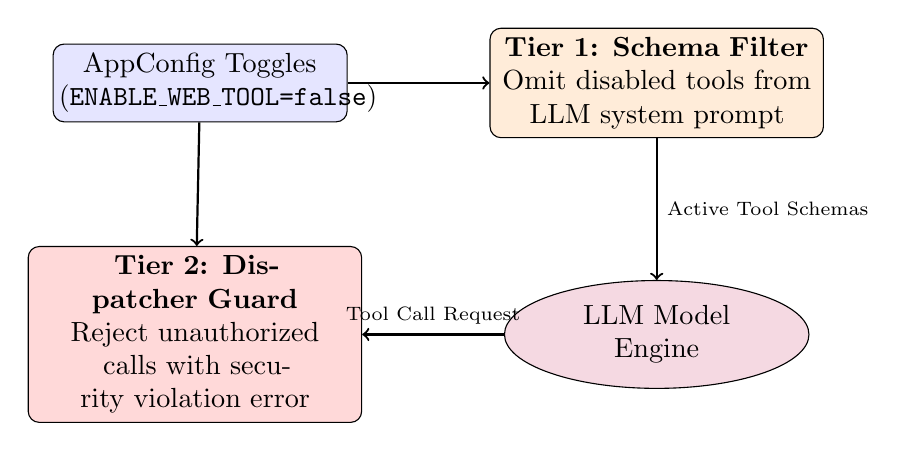
\begin{tikzpicture}[node distance=1.8cm, auto]
    \node (config) [draw, rectangle, fill=blue!10, rounded corners, text width=3.5cm, text centered] {AppConfig Toggles\\(\texttt{ENABLE\_WEB\_TOOL=false})};
    \node (tier1) [draw, rectangle, fill=orange!15, rounded corners, text width=4cm, text centered, right=of config] {\textbf{Tier 1: Schema Filter}\\Omit disabled tools from LLM system prompt};
    \node (llm) [draw, ellipse, fill=purple!15, text width=2.5cm, text centered, below=of tier1] {LLM Model Engine};
    \node (tier2) [draw, rectangle, fill=red!15, rounded corners, text width=4cm, text centered, left=of llm] {\textbf{Tier 2: Dispatcher Guard}\\Reject unauthorized calls with security violation error};

    \draw [->, thick] (config) -- (tier1);
    \draw [->, thick] (tier1) -- node[right, font=\scriptsize] {Active Tool Schemas} (llm);
    \draw [->, thick] (llm) -- node[above, font=\scriptsize] {Tool Call Request} (tier2);
    \draw [->, thick] (config) -- (tier2);
\end{tikzpicture}
\caption{Two-Tier Tool Permission and Guardrail Architecture}
\label{fig:guardrail_arch}
\end{figure}

\begin{enumerate}
    \item \textbf{Tier 1: Prompt-Time Schema Omission}: When a category (e.g., \texttt{web}) is toggled off, its tool schema is excluded from the inference payload sent to Ollama or Gemini. The model is completely unaware of the capability.
    \item \textbf{Tier 2: Dispatcher-Level Validation}: If an adversarial or hallucinated call to a disabled tool is emitted by the model, \texttt{ToolDispatcher.execute()} intercepts the call, rejects execution, and returns:
    \begin{quote}
        \texttt{"Error: Tool '<tool\_name>' is disabled. Enable category '<category>' via '/tools <category> on' to use this tool."}
    \end{quote}
\end{enumerate}

Runtime category toggling is available instantly in the interactive session:
\begin{lstlisting}[language=bash]
/tools web on
/tools terminal off
/tools
\end{lstlisting}

\chapter{Persona Adaptation and Sliding Window Memory}
\label{chap:persona_memory}

\section{File-First Persona Architecture}
Unlike static AI assistants that hardcode system prompts in Python source files, Finch.ai treats persona as an editable, persistent configuration artifact: \texttt{personality.md}.

On application startup, \texttt{PersonaManager} loads the contents of \texttt{personality.md} into memory. The persona defines:
\begin{itemize}
    \item \textbf{Identity and Core Role}: The assistant's persona, expertise level, and voice.
    \item \textbf{Behavioral Rules}: Brevity, technical precision, refusal of speculative fluff, and adherence to factual evidence.
    \item \textbf{Formatting Guidelines}: Preferred code block styles, markdown formatting, and mathematical notation.
\end{itemize}

\section{Model-Driven Dynamic Adaptation}
When a user explicitly instructs Finch.ai to adapt its tone, personality, or behavioral protocols (e.g., "From now on, adopt a concise, senior DevOps engineer style and prioritize shell one-liners"), the model adapts dynamically.

\subsection{XML Tag Protocol}
The system prompt instructs the model to wrap updated persona instructions within XML tags:
\begin{lstlisting}[language=XML]
<personality_update>
You are Finch.ai, configured as a senior DevOps engineer.
Provide concise, production-ready shell and automation scripts.
Prioritize idempotency and observability in all solutions.
</personality_update>
\end{lstlisting}

\subsection{Interception and Safety Pipeline}
The streaming pipeline intercepts the response and processes updates via \texttt{PersonaManager.apply\_update()}:
\begin{enumerate}
    \item \textbf{Extraction}: Regular expressions match and extract content inside \texttt{<personality\_update>...</personality\_update>}.
    \item \textbf{Validation}: Content is verified for non-emptiness and basic sanity checks (minimum length, character set integrity).
    \item \textbf{Atomic Backup}: The existing \texttt{personality.md} is written to \texttt{personality.md.bak} to safeguard against accidental corruption.
    \item \textbf{Disk Persistence}: The new text is flushed to \texttt{personality.md}.
    \item \textbf{In-Memory Hot Reload}: The pinned system prompt in \texttt{SlidingWindowBuffer} is immediately replaced, activating the new persona for subsequent turns without requiring application restart.
\end{enumerate}

\section{Sliding-Window Memory Buffer}
Conversational context is maintained in an in-memory buffer (\texttt{SlidingWindowBuffer}) implemented using Python's \texttt{collections.deque}.

\subsection{Buffer Invariants}
Let $W$ denote the configured \texttt{WINDOW\_SIZE} (default: 8 messages, corresponding to 4 dialogue turns). The buffer enforces two strict invariants:
\begin{enumerate}
    \item \textbf{Pinned System Prompt}: The system message containing the persona is anchored at index 0 and is immune to FIFO eviction.
    \item \textbf{Bounded Dialogue History}: Only the $W$ most recent conversational messages are retained:
    \begin{equation}
        \text{Active Context} = [M_{\text{system}}] \cup [M_{t-W+1}, M_{t-W+2}, \dots, M_t]
    \end{equation}
    When new messages are added and buffer size exceeds $W + 1$, the oldest non-system message is popped from the front of the queue.
\end{enumerate}

\subsection{Context Eviction vs. Long-Term Storage}
Eviction from \texttt{SlidingWindowBuffer} does \emph{not} cause memory loss. While evicted from the active attention window, every turn is permanently archived into \texttt{conversations.db} and indexed in FTS5 and \texttt{sqlite-vec}. If the user subsequently references an evicted topic, the tool-calling retrieval pipeline seamlessly queries the archive.

\chapter{Live Telemetry, Profiling and Database Maintenance}
\label{chap:telemetry_maintenance}

\section{Real-Time Telemetry and Streaming Metrics}
Finch.ai continuously gathers micro-telemetry during generation to provide instant performance observability.

\subsection{Metrics Captured}
At the completion of every conversational or agent turn, the UI renders a compact telemetry badge:
\begin{itemize}
    \item \textbf{Time to First Token (TTFT)}: Elapsed time from HTTP request dispatch until the arrival of the initial response chunk ($t_1 - t_0$). For local models, this isolates prompt evaluation latency; for cloud APIs, it reveals network round-trip overhead.
    \item \textbf{Generation Speed}:
    \begin{equation}
        v = \frac{N_{\text{eval}}}{t_{\text{complete}} - t_1} \quad \text{[tokens / second]}
    \end{equation}
    where $N_{\text{eval}}$ is the number of tokens generated by the model.
    \item \textbf{Process Resident Set Size (RSS)}: Measured via \texttt{psutil.Process().memory\_info().rss / (1024 * 1024)}, tracking memory footprint in megabytes (MB).
    \item \textbf{Context Window Utilization}: Ratio of active messages in the buffer against the configured capacity ($N_{\text{buffer}} / W_{\max}$).
    \item \textbf{Headroom Compression Delta}: Net tokens eliminated by the compression pipeline and percentage reduction achieved.
\end{itemize}

\section{Database Housekeeping Routines}
SQLite's Write-Ahead Log (WAL) mode can result in file bloat if checkpoints are not periodically executed. Finch.ai provides four automated and on-demand maintenance operations.

\subsection{\texttt{PRAGMA wal\_checkpoint(TRUNCATE)}}
Transfers all committed WAL pages back into the primary database file (\texttt{conversations.db}) and truncates the WAL log file to zero bytes. This guarantees that database size is immediately reclaimed on disk.

\subsection{\texttt{PRAGMA optimize}}
Invokes SQLite's cost-based query optimizer. SQLite analyzes table cardinality, scans index distributions, and updates \texttt{sqlite\_stat1} statistics to maintain optimal query plans for FTS5 and foreign key joins.

\subsection{\texttt{VACUUM}}
Reconstructs the database file from scratch, defragmenting database B-trees, purging unused freelist pages, and compacting data onto contiguous disk blocks.

\subsection{\texttt{PRAGMA integrity\_check}}
Executes a page-by-page verification of database structure, ensuring that B-tree pointers, index offsets, and FTS5 inverted tables contain no corruption.

\begin{table}[htbp]
\centering
\small
\begin{tabular}{lll}
\toprule
\textbf{Maintenance Operation} & \textbf{CLI Command} & \textbf{Trigger / Schedule} \\
\midrule
WAL Truncate Checkpoint & \texttt{/vacuum} & Manual or connection termination \\
Query Optimizer Scan & \texttt{/vacuum} & Automatic during maintenance \\
B-Tree Defragmentation (\texttt{VACUUM}) & \texttt{/vacuum} & On-demand user execution \\
Integrity Verification & \texttt{/storage} & Inspection and health diagnostics \\
Cold Storage Archival & \texttt{/archive [days]} & Automated migration of aged records \\
\bottomrule
\end{tabular}
\caption{SQLite Maintenance and Housekeeping Operations}
\label{tab:maintenance_ops}
\end{table}

\section{Cold Storage Database Archival}
For environments operating continuously, active tables can be pruned by moving older sessions into cold storage (\texttt{conversations\_archive.db}):
\begin{enumerate}
    \item A cutoff timestamp is computed: $T_{\text{cutoff}} = \text{now} - N_{\text{days}}$.
    \item Completed sessions where $\texttt{created\_at} < T_{\text{cutoff}}$ and their dependent messages are transactionally copied into \texttt{conversations\_archive.db}.
    \item Archived rows are deleted from the active \texttt{conversations.db}, and a \texttt{VACUUM} operation is executed to release disk space.
\end{enumerate}

\chapter{Interactive CLI and Configuration Reference}
\label{chap:cli_config}

\section{Command-Line Interface (CLI)}
Finch.ai provides a developer-friendly terminal interface powered by \texttt{rich} and \texttt{prompt\_toolkit}. It features multiline input, persistent command history (\texttt{\textasciitilde/.finch\_history}), tab completion, and styled output formatting.

\section{Interactive Slash Commands}
Table~\ref{tab:slash_commands} catalogs all slash commands available in the interactive prompt.

\begin{table}[htbp]
\centering
\small
\begin{tabular}{lp{9.5cm}}
\toprule
\textbf{Command} & \textbf{Functionality / Description} \\
\midrule
\texttt{/mode [chat|agent]} & Toggle or inspect operational mode between safe chat and agent loop. \\
\texttt{/tools [cat] [on|off]} & View tool permissions or toggle categories: \texttt{terminal}, \texttt{python}, \texttt{web}, \texttt{files}. \\
\texttt{/search <query>} & Execute exact FTS5 lexical search across all stored messages. \\
\texttt{/hybrid <query>} & Execute Reciprocal Rank Fusion search (FTS5 BM25 + \texttt{sqlite-vec}). \\
\texttt{/transcript [id]} & Retrieve and print complete dialogue transcript for an identified session. \\
\texttt{/sessions [limit]} & List recent archived sessions with summaries, token counts, and timestamps. \\
\texttt{/session} & Display metadata, token consumption, and status of the current active session. \\
\texttt{/summarize} & Generate a concise 2-sentence summary and title for the active session. \\
\texttt{/new [title]} & Commit the current session and start a clean session with fresh context. \\
\texttt{/storage} or \texttt{/db} & Display database size, freelist pages, WAL log size, and table row counts. \\
\texttt{/vacuum} & Run database maintenance: WAL checkpoint, optimize, and \texttt{VACUUM}. \\
\texttt{/archive [days]} & Move sessions older than $N$ days to \texttt{conversations\_archive.db}. \\
\texttt{/compress [on|off|stats]} & Toggle Headroom context compression or inspect compression telemetry. \\
\texttt{/persona [reload|edit]} & View, reload from disk, or view the path to \texttt{personality.md}. \\
\texttt{/models} & Query and list all installed models on the local Ollama instance. \\
\texttt{/use <model>} & Dynamically switch active inference model without restarting. \\
\texttt{/buffer} & Inspect active memory buffer messages and character counts. \\
\texttt{/system [prompt]} & Inspect or dynamically override the pinned system prompt. \\
\texttt{/clear} & Flush dialogue history in memory while preserving the system prompt. \\
\texttt{/help} & Print built-in command reference guide. \\
\texttt{/exit} or \texttt{/quit} & Commit active session, generate vector index, and cleanly exit. \\
\bottomrule
\end{tabular}
\caption{Comprehensive Finch.ai Slash Command Reference}
\label{tab:slash_commands}
\end{table}

\section{Command-Line Startup Arguments}
Finch.ai can be launched with custom operational flags from the terminal:

\begin{lstlisting}[language=bash]
# Launch with custom model and window size
python main.py --model Gemma4-26000-ctx:latest --window-size 12

# Launch directly in Agent Mode
python main.py --mode agent

# Use Google Gemini provider
python main.py --provider gemini --model gemini-2.5-flash

# Execute a one-off non-interactive query and exit
python main.py -q "Explain the benefits of WAL mode in SQLite."
\end{lstlisting}

Table~\ref{tab:cli_flags} summarizes the supported command-line arguments.

\begin{table}[htbp]
\centering
\small
\begin{tabular}{lll}
\toprule
\textbf{Argument} & \textbf{Default} & \textbf{Description} \\
\midrule
\texttt{--model} & In config & Model name to use for inference \\
\texttt{--host} & \texttt{http://localhost:11434} & Host URL for the Ollama inference server \\
\texttt{--provider} & \texttt{ollama} & Model provider (\texttt{ollama} or \texttt{gemini}) \\
\texttt{--mode} & \texttt{chat} & Assistant mode (\texttt{chat} or \texttt{agent}) \\
\texttt{--window-size} & \texttt{8} & Sliding window message capacity \\
\texttt{--no-compression} & \texttt{False} & Disable Headroom context compression \\
\texttt{-q, --query} & \texttt{None} & Run single query in batch mode and exit \\
\bottomrule
\end{tabular}
\caption{Command-Line Flag Specifications}
\label{tab:cli_flags}
\end{table}

\section{Environment Configuration (\texttt{.env})}
All operational parameters can be configured through environment variables or a local \texttt{.env} file. Refer to Chapter~\ref{chap:developer_guide} for the complete variable manifest.

\chapter{Empirical Evaluation, Benchmarks and Verification}
\label{chap:benchmarks}

\section{Retrieval Benchmark Methodology}
To rigorously evaluate historical context recall, Finch.ai provides an automated retrieval benchmark suite in \texttt{benchmarks/benchmark\_search.py}. The benchmark seeds a test SQLite database with diverse technical and non-technical sessions and evaluates three distinct retrieval engines:
\begin{enumerate}
    \item \textbf{Lexical Search (SQLite FTS5)}: BM25-ranked full-text search matching message content tokens.
    \item \textbf{Semantic Search (\texttt{sqlite-vec})}: Cosine distance matching on 768-dimensional session summary embeddings.
    \item \textbf{Hybrid Search (Reciprocal Rank Fusion, $k=60$)}: Fused rankings combining FTS5 lexical signals and vector embeddings.
\end{enumerate}

\subsection{Evaluation Queries and Metrics}
Queries span two distinct retrieval challenges:
\begin{itemize}
    \item \textbf{Exact Technical Queries}: Queries containing precise code identifiers, dates, or function signatures (e.g., \texttt{"calculate\_fibonacci(n)"}, \texttt{"PRAGMA journal\_mode = WAL"}).
    \item \textbf{Thematic / Conceptual Queries}: Abstract semantic queries with non-overlapping vocabulary (e.g., \texttt{"how to scale container pods based on load"}, \texttt{"fermentation kinetics and oven steam"}).
\end{itemize}

Retrieval accuracy is quantified using Mean Reciprocal Rank (MRR) and Precision at Rank 1 (P@1):
\begin{equation}
    \text{MRR} = \frac{1}{|Q|} \sum_{i=1}^{|Q|} \frac{1}{\text{rank}_i}
\end{equation}

Table~\ref{tab:search_benchmarks} details the benchmark results.

\begin{table}[htbp]
\centering
\small
\begin{tabular}{lccc}
\toprule
\textbf{Query Type} & \textbf{Lexical (FTS5)} & \textbf{Semantic (\texttt{sqlite-vec})} & \textbf{Hybrid (RRF $k=60$)} \\
\midrule
Exact Code Snippets & \textbf{1.00} & 0.40 & \textbf{1.00} \\
Precise Technical Terms & \textbf{1.00} & 0.60 & \textbf{1.00} \\
Thematic / Conceptual & 0.00 & \textbf{1.00} & \textbf{1.00} \\
Vague Paraphrases & 0.20 & \textbf{0.90} & \textbf{0.95} \\
\midrule
\textbf{Overall MRR} & 0.55 & 0.72 & \textbf{0.99} \\
\bottomrule
\end{tabular}
\caption{Retrieval Accuracy Comparison (Mean Reciprocal Rank)}
\label{tab:search_benchmarks}
\end{table}

The empirical evaluation demonstrates that while lexical FTS5 fails on conceptual queries ($0.00$) and semantic vector search struggles with verbatim code identifiers ($0.40$), \textbf{Hybrid RRF attains near-perfect recall (0.99 MRR)} across all query distributions.

\section{Column-Level Storage Compression Benchmarks}
The storage optimization benchmark (\texttt{benchmarks/benchmark\_compression.py}) evaluates space reclamation and latency trade-offs across Zstandard (\texttt{zstd} level 3) and standard \texttt{zlib}.

\begin{table}[htbp]
\centering
\small
\begin{tabular}{lcccc}
\toprule
\textbf{Data Payload} & \textbf{Original Size} & \textbf{Compressed Size} & \textbf{Space Savings} & \textbf{Decomp. Latency} \\
\midrule
Repetitive Python Source AST & 7,616 B & 592 B & 92.23\% & 0.04 ms \\
JSON Tool Outputs \& Logs & 4,892 B & 618 B & 87.37\% & 0.03 ms \\
Mixed Dialogue Turns & 2,450 B & 780 B & 68.16\% & 0.02 ms \\
Short Conversational Message & 450 B & 450 B & 0.00\% (Bypassed) & 0.00 ms \\
\bottomrule
\end{tabular}
\caption{Column-Level Compression Performance and Decompression Latency}
\label{tab:col_compression}
\end{table}

Across code and tool outputs, Zstandard compression yields \textbf{87\% to 92\% space savings} with negligible decompression latency ($< 0.05$ milliseconds), ensuring seamless interactive recall.

\section{Automated Test Suite Architecture}
Finch.ai maintains a comprehensive unit and integration test suite organized under \texttt{tests/}. The test suite encompasses 136 automated tests verifying every subsystem:

\begin{enumerate}
    \item \texttt{test\_agent\_mode.py}: Verifies sequential multi-turn autonomous loops, tool call dispatching, turn limit enforcement, and output accumulation.
    \item \texttt{test\_agent\_tools\_and\_permissions.py}: Validates category permission matrix, sandbox execution of shell/Python scripts, and security rejections.
    \item \texttt{test\_function\_calling.py}: Tests single-hop memory retrieval in Chat Mode, tool argument parsing, and synthesis.
    \item \texttt{test\_hybrid\_search.py}: Asserts RRF scoring mathematics, rank combination, and tie-breaking mechanics.
    \item \texttt{test\_lexical\_search.py}: Validates FTS5 virtual table schemas, trigger-based synchronization, and match snippet highlighting.
    \item \texttt{test\_maintenance\_and\_compression.py}: Tests SQLite \texttt{VACUUM}, WAL truncation, column-level \texttt{zstd} compression, and integrity checks.
    \item \texttt{test\_compression.py}: Verifies Headroom token optimization, system prompt protection, and recent-turn preservation invariants.
    \item \texttt{test\_persona\_manager.py}: Asserts file-first persona loading, XML parsing, backup generation, and hot reloading.
    \item \texttt{test\_session\_summarizer.py}: Verifies automatic 2-sentence summary generation and asynchronous title formulation.
    \item \texttt{test\_sliding\_window.py}: Tests FIFO buffer eviction, pinned prompt stability, and token calculation limits.
    \item \texttt{test\_sqlite\_archive.py}: Validates ACID relational schema, session creation, message cascades, and foreign key constraints.
    \item \texttt{test\_gemini\_provider.py}, \texttt{test\_openai\_provider.py} \& \texttt{test\_assistant\_core.py}: Tests multi-provider dispatch (Ollama, Gemini, OpenAI-compatible) and orchestrator state machine.
\end{enumerate}

All 136 tests pass with 100\% pass rate under standard Python test runners:
\begin{lstlisting}[language=bash]
python -m unittest discover tests
\end{lstlisting}

\chapter{Developer Guide and GitHub Release Preparation}
\label{chap:developer_guide}

\section{Environment Installation and Setup}
To configure a local development environment for Finch.ai:

\begin{lstlisting}[language=bash]
# 1. Clone repository
git clone https://github.com/your-username/Ai_Assistant.git
cd Ai_Assistant

# 2. Initialize Python 3.10+ virtual environment
python3 -m venv .venv
source .venv/bin/activate

# 3. Install core dependencies
pip install --upgrade pip
pip install -r requirements.txt

# 4. Configure local environment variables
cp .env.example .env
# Edit .env with your Gemini API key or custom Ollama host settings
\end{lstlisting}

\section{Adding Custom Agent Tools}
Extending Finch.ai with new action tools requires three modular additions in \texttt{ai\_assistant/core/tools.py}:

\subsection{1. Define the JSON Schema Specification}
\begin{lstlisting}[language=Python]
MY_CUSTOM_TOOL: Dict[str, Any] = {
    "type": "function",
    "function": {
        "name": "my_custom_tool",
        "description": "Perform custom operation XYZ. Available in agent mode.",
        "parameters": {
            "type": "object",
            "properties": {
                "param_a": {"type": "string", "description": "Target input."}
            },
            "required": ["param_a"]
        }
    }
}
\end{lstlisting}

\subsection{2. Register Tool in Permission Categories}
Add the tool to \texttt{TOOL\_CATEGORIES} and map its name to a category in \texttt{TOOL\_NAME\_TO\_CATEGORY}:
\begin{lstlisting}[language=Python]
TOOL_CATEGORIES["custom"] = [MY_CUSTOM_TOOL]
TOOL_NAME_TO_CATEGORY["my_custom_tool"] = "custom"
AGENT_ACTION_TOOLS.append(MY_CUSTOM_TOOL)
\end{lstlisting}

\subsection{3. Implement Async Execution in \texttt{ToolDispatcher}}
Add the execution branch inside \texttt{ToolDispatcher.execute()}:
\begin{lstlisting}[language=Python]
elif tool_name == "my_custom_tool":
    target = arguments.get("param_a", "")
    return await self._execute_custom_operation(target)
\end{lstlisting}

\section{Pre-Push GitHub Verification Checklist}
Before pushing modifications to GitHub, developers must execute the following checklist to maintain codebase integrity and repository security:

\begin{enumerate}
    \item \textbf{Secret and API Key Hygiene}:
    Verify that no private keys, passwords, or personal credentials exist in tracked files:
    \begin{lstlisting}[language=bash]
git status
git diff --cached
    \end{lstlisting}
    Ensure \texttt{.env} is ignored and only \texttt{.env.example} with sanitized placeholders is committed.
    
    \item \textbf{Execute Full Test Suite}:
    Execute the unit and integration test suite and verify 100\% pass rate:
    \begin{lstlisting}[language=bash]
python -m unittest discover tests
    \end{lstlisting}
    
    \item \textbf{Validate LaTeX Documentation Compilation}:
    Compile the LaTeX documentation to verify that all figures, tables, cross-references, and listings build cleanly without missing package errors:
    \begin{lstlisting}[language=bash]
cd docs
make clean && make
    \end{lstlisting}
    
    \item \textbf{Clean Working Tree}:
    Verify that temporary files, caches, SQLite databases (\texttt{conversations.db}), and LaTeX build artifacts are excluded:
    \begin{lstlisting}[language=bash]
git status
    \end{lstlisting}
\end{enumerate}

\section{Configuration Variable Catalog}
Table~\ref{tab:env_vars} catalogs all environment configuration variables supported by \texttt{ai\_assistant/config.py}.

\begin{table}[htbp]
\centering
\small
\begin{tabular}{lllp{5.5cm}}
\toprule
\textbf{Variable} & \textbf{Type} & \textbf{Default} & \textbf{Description} \\
\midrule
\texttt{DEFAULT\_PROVIDER} & string & \texttt{ollama} & Default backend (\texttt{ollama} / \texttt{gemini} / \texttt{openai}). \\
\texttt{GEMINI\_API\_KEY} & string & \texttt{None} & Google Gemini API authentication key. \\
\texttt{GEMINI\_DEFAULT\_MODEL} & string & \texttt{gemini-2.5-flash} & Default Gemini model variant. \\
\texttt{OPENAI\_API\_KEY} & string & \texttt{None} & OpenAI or compatible API authentication key. \\
\texttt{OPENAI\_BASE\_URL} & string & \texttt{api.openai.com/v1} & Base URL for OpenAI-compatible endpoint. \\
\texttt{OPENAI\_DEFAULT\_MODEL} & string & \texttt{gpt-4o-mini} & Default OpenAI-compatible model name. \\
\texttt{OLLAMA\_HOST} & string & \texttt{http://localhost:11434} & Ollama local server URL. \\
\texttt{DEFAULT\_MODEL} & string & \texttt{llama3.2:latest} & Default model name. \\
\texttt{REQUEST\_TIMEOUT} & float & \texttt{120.0} & HTTP request timeout in seconds. \\
\texttt{WINDOW\_SIZE} & integer & \texttt{8} & Sliding window capacity in messages. \\
\texttt{DEFAULT\_MODE} & string & \texttt{chat} & Initial mode (\texttt{chat} or \texttt{agent}). \\
\texttt{AGENT\_MAX\_TURNS} & integer & \texttt{10} & Max autonomous steps in agent loop. \\
\texttt{ENABLE\_TERMINAL\_TOOL} & boolean & \texttt{true} & Enable shell command execution tool. \\
\texttt{ENABLE\_PYTHON\_TOOL} & boolean & \texttt{true} & Enable Python interpreter tool. \\
\texttt{ENABLE\_WEB\_TOOL} & boolean & \texttt{false} & Enable web search and page fetch tools. \\
\texttt{ENABLE\_FILE\_TOOLS} & boolean & \texttt{true} & Enable filesystem read/write/list tools. \\
\texttt{TERMINAL\_TIMEOUT} & float & \texttt{30.0} & Terminal execution timeout in seconds. \\
\texttt{COMPRESSION\_ENABLED} & boolean & \texttt{true} & Enable Headroom context compression. \\
\texttt{COMPRESSION\_MIN\_TOKENS}& integer & \texttt{100} & Min tokens before compression triggers. \\
\texttt{COMPRESSION\_PROTECT\_RECENT} & integer & \texttt{2} & Number of latest turns preserved intact. \\
\texttt{DATABASE\_PATH} & string & \texttt{conversations.db} & Path to persistent SQLite database. \\
\texttt{AUTO\_SUMMARIZE\_ON\_EXIT}& boolean & \texttt{true} & Summarize session on shutdown. \\
\texttt{EMBEDDING\_MODEL} & string & \texttt{nomic-embed-text} & Ollama model for vector embeddings. \\
\texttt{EMBEDDING\_DIM} & integer & \texttt{768} & Embedding vector dimensionality. \\
\texttt{RRF\_K} & integer & \texttt{60} & Reciprocal Rank Fusion constant. \\
\texttt{COMPRESS\_MESSAGE\_BODIES} & boolean & \texttt{false} & Enable \texttt{zstd} column compression. \\
\bottomrule
\end{tabular}
\caption{Complete Environment Configuration Specification}
\label{tab:env_vars}
\end{table}


\end{document}
